\documentclass[11pt, halfparskip]{article}
%\usepackage[T1]{fontenc}
%\usepackage{helvet}

\usepackage{tikz}


\definecolor{tocheck}{RGB}{255, 140, 0}
\definecolor{checked}{RGB}{19, 178, 61}
\definecolor{currentfocus}{RGB}{0, 102, 219}
\begin{document}
	% Needed colors
	% To check: orange
	% Checked: green
	% Current focus: blue
	
	% Looking for element 21
	\noindent
	Let's look at the following array with 10 elements. The indices go from 0 as the first to 9 as the last element.
	\\
	Our goal is to find out, if the array contains the element 5.
	\begin{center}
		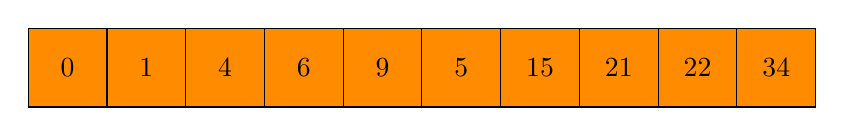
\begin{tikzpicture}
			\filldraw [draw=black, fill=tocheck] (0, 0) rectangle (1, 1) node[midway]{0};
			\filldraw [draw=black, fill=tocheck] (1, 0) rectangle (2, 1) node[midway]{1};
			\filldraw [draw=black, fill=tocheck] (2, 0) rectangle (3, 1) node[midway]{4};
			\filldraw [draw=black, fill=tocheck] (3, 0) rectangle (4, 1) node[midway]{6};
			\filldraw [draw=black, fill=tocheck] (4, 0) rectangle (5, 1) node[midway]{9};
			\filldraw [draw=black, fill=tocheck] (5, 0) rectangle (6, 1) node[midway]{5};
			\filldraw [draw=black, fill=tocheck] (6, 0) rectangle (7, 1) node[midway]{15};
			\filldraw [draw=black, fill=tocheck] (7, 0) rectangle (8, 1) node[midway]{21};
			\filldraw [draw=black, fill=tocheck] (8, 0) rectangle (9, 1) node[midway]{22};
			\filldraw [draw=black, fill=tocheck] (9, 0) rectangle (10, 1) node[midway]{34};
		\end{tikzpicture}
	\end{center}
	
	\noindent \\
	First we need to find the middle of our array. Our maximum index is 9 so half would be 4.5. Since only integers can be indices, let's round this to 4.
	\\
	So the element we are currently looking for has index 4 and to make things easier, let's call this the pivot element. In our array the pivot element has
	the value 9 (highlighted blue below).
	\begin{center}
		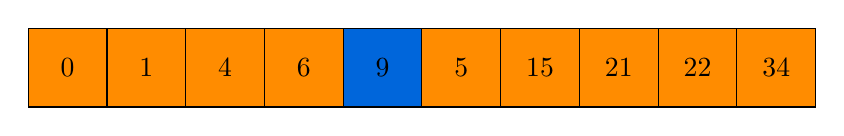
\begin{tikzpicture}
			\filldraw [draw=black, fill=tocheck] (0, 0) rectangle (1, 1) node[midway]{0};
			\filldraw [draw=black, fill=tocheck] (1, 0) rectangle (2, 1) node[midway]{1};
			\filldraw [draw=black, fill=tocheck] (2, 0) rectangle (3, 1) node[midway]{4};
			\filldraw [draw=black, fill=tocheck] (3, 0) rectangle (4, 1) node[midway]{6};
			\filldraw [draw=black, fill=currentfocus] (4, 0) rectangle (5, 1) node[midway]{9};
			\filldraw [draw=black, fill=tocheck] (5, 0) rectangle (6, 1) node[midway]{5};
			\filldraw [draw=black, fill=tocheck] (6, 0) rectangle (7, 1) node[midway]{15};
			\filldraw [draw=black, fill=tocheck] (7, 0) rectangle (8, 1) node[midway]{21};
			\filldraw [draw=black, fill=tocheck] (8, 0) rectangle (9, 1) node[midway]{22};
			\filldraw [draw=black, fill=tocheck] (9, 0) rectangle (10, 1) node[midway]{34};
		\end{tikzpicture}
	\end{center}
	
	\noindent \\
	Our pivot is not equal to 5, so we haven't reached our goal yet. But since the list is sorted and 9 is less than 5, we know that both the pivot and
	everything on it's right side can not contain 5.
	\\
	This reduces the amount of elements we need to care about from 10 to 5.
	\begin{center}
		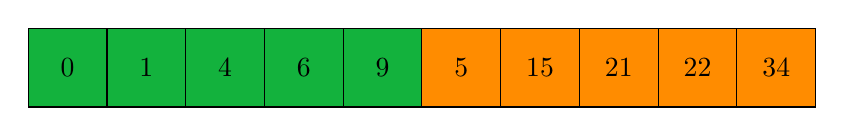
\begin{tikzpicture}
			\filldraw [draw=black, fill=checked] (0, 0) rectangle (1, 1) node[midway]{0};
			\filldraw [draw=black, fill=checked] (1, 0) rectangle (2, 1) node[midway]{1};
			\filldraw [draw=black, fill=checked] (2, 0) rectangle (3, 1) node[midway]{4};
			\filldraw [draw=black, fill=checked] (3, 0) rectangle (4, 1) node[midway]{6};
			\filldraw [draw=black, fill=checked] (4, 0) rectangle (5, 1) node[midway]{9};
			\filldraw [draw=black, fill=tocheck] (5, 0) rectangle (6, 1) node[midway]{5};
			\filldraw [draw=black, fill=tocheck] (6, 0) rectangle (7, 1) node[midway]{15};
			\filldraw [draw=black, fill=tocheck] (7, 0) rectangle (8, 1) node[midway]{21};
			\filldraw [draw=black, fill=tocheck] (8, 0) rectangle (9, 1) node[midway]{22};
			\filldraw [draw=black, fill=tocheck] (9, 0) rectangle (10, 1) node[midway]{34};
		\end{tikzpicture}
	\end{center}
	
	\noindent \\
	Now we have 5 elements left and want to check the rest of the array for 5. First we need to find the pivot element again. If we only looked at the
	last 5 elements we would go from index 0-4 and our pivot element therefore would have index 2. But since we need to take the previously checked elements
	into account, we have to add the length of the already checked array.
	\\
	5+2 = 7 so our pivot element is at index 7 and has the value 21.
	\begin{center}
		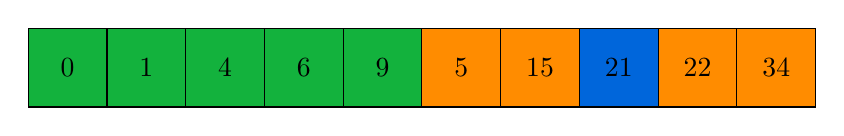
\begin{tikzpicture}
			\filldraw [draw=black, fill=checked] (0, 0) rectangle (1, 1) node[midway]{0};
			\filldraw [draw=black, fill=checked] (1, 0) rectangle (2, 1) node[midway]{1};
			\filldraw [draw=black, fill=checked] (2, 0) rectangle (3, 1) node[midway]{4};
			\filldraw [draw=black, fill=checked] (3, 0) rectangle (4, 1) node[midway]{6};
			\filldraw [draw=black, fill=checked] (4, 0) rectangle (5, 1) node[midway]{9};
			\filldraw [draw=black, fill=tocheck] (5, 0) rectangle (6, 1) node[midway]{5};
			\filldraw [draw=black, fill=tocheck] (6, 0) rectangle (7, 1) node[midway]{15};
			\filldraw [draw=black, fill=currentfocus] (7, 0) rectangle (8, 1) node[midway]{21};
			\filldraw [draw=black, fill=tocheck] (8, 0) rectangle (9, 1) node[midway]{22};
			\filldraw [draw=black, fill=tocheck] (9, 0) rectangle (10, 1) node[midway]{34};
		\end{tikzpicture}
	\end{center}
	
	\newpage
	\noindent \\
	21 is still not equal to 5, but we since it is higher, we know that we can ignore everything on the right side. Again, this only works if the array is sorted.
	\begin{center}
		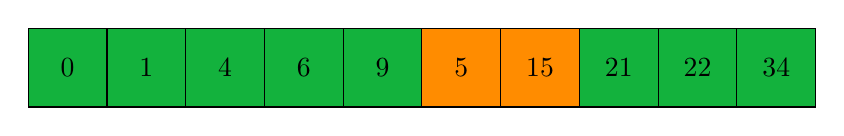
\begin{tikzpicture}
			\filldraw [draw=black, fill=checked] (0, 0) rectangle (1, 1) node[midway]{0};
			\filldraw [draw=black, fill=checked] (1, 0) rectangle (2, 1) node[midway]{1};
			\filldraw [draw=black, fill=checked] (2, 0) rectangle (3, 1) node[midway]{4};
			\filldraw [draw=black, fill=checked] (3, 0) rectangle (4, 1) node[midway]{6};
			\filldraw [draw=black, fill=checked] (4, 0) rectangle (5, 1) node[midway]{9};
			\filldraw [draw=black, fill=tocheck] (5, 0) rectangle (6, 1) node[midway]{5};
			\filldraw [draw=black, fill=tocheck] (6, 0) rectangle (7, 1) node[midway]{15};
			\filldraw [draw=black, fill=checked] (7, 0) rectangle (8, 1) node[midway]{21};
			\filldraw [draw=black, fill=checked] (8, 0) rectangle (9, 1) node[midway]{22};
			\filldraw [draw=black, fill=checked] (9, 0) rectangle (10, 1) node[midway]{34};
		\end{tikzpicture}
	\end{center}
	
	\noindent \\
	Looking for our pivot element again we find it has index 5. We check the element at this position and see that this equals the element we were looking for.
	\begin{center}
		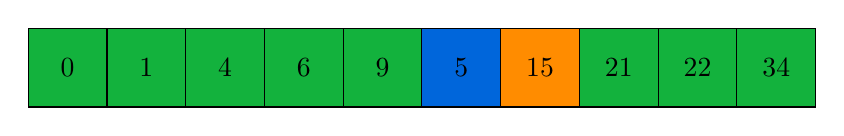
\begin{tikzpicture}
			\filldraw [draw=black, fill=checked] (0, 0) rectangle (1, 1) node[midway]{0};
			\filldraw [draw=black, fill=checked] (1, 0) rectangle (2, 1) node[midway]{1};
			\filldraw [draw=black, fill=checked] (2, 0) rectangle (3, 1) node[midway]{4};
			\filldraw [draw=black, fill=checked] (3, 0) rectangle (4, 1) node[midway]{6};
			\filldraw [draw=black, fill=checked] (4, 0) rectangle (5, 1) node[midway]{9};
			\filldraw [draw=black, fill=currentfocus] (5, 0) rectangle (6, 1) node[midway]{5};
			\filldraw [draw=black, fill=tocheck] (6, 0) rectangle (7, 1) node[midway]{15};
			\filldraw [draw=black, fill=checked] (7, 0) rectangle (8, 1) node[midway]{21};
			\filldraw [draw=black, fill=checked] (8, 0) rectangle (9, 1) node[midway]{22};
			\filldraw [draw=black, fill=checked] (9, 0) rectangle (10, 1) node[midway]{34};
		\end{tikzpicture}
	\end{center}
	
	\noindent \\
	Now we are done and it only took 3 steps. If we were to search for the element by going through the entire array, it would have taken us 6 steps.
	\\
	While this is already double, it still seems little, but for big arrays, the amount of steps for just going through the list grow substantially, while with using binary
	search the steps remain pretty low.
\end{document}